\section{Продложение потоков. Алгоритм Диница, теоремы Карзанова}%
\label{sec:Продложение потоков. Алгоритм Диница, теоремы Карзанова}

\subsection{Детали реализации.}%
\label{sub:Детали реализации.}


\begin{lstlisting}[mathescape, language = C++, caption = Удобная реализация ребер, escapeinside={\%*}{*}] 
	struct Edge {
		int from = 0,
		    to   = 0;

		long long cap = 0;
		long long flow = 0;
	};

	auto edges = vector<Edge>();
	auto outbound = vector<vector<int>>(); 
	/* v-th element -- numbers of edges from v. */
\end{lstlisting}

Рядом с каждым ребром всегда есть обратное, изначально с нулевой capacity. Будем присваивать обратному ребру номер исходного, увеличенный на 1. К примеру номера $2n$ и $2n + 1$.
Тогда при добавлении нового ребра в граф, мы будем добавлять его и сразу же добавлять обратное, а потом сохранять номера обоих ребер в массив edges.

Теперь если мы пускаем поток по ребру с номером $i$, то можем удобно уменьшить поток по противоположному ребру, как имеющее номер $i \oplus 1$

\begin{lstlisting}[language = C++]
	edges[i].flow	 += delta_flow;
	edges[i ^ 1].flow -= delta_flow;
\end{lstlisting}
При реализации алгоритма Форда-Фалкерсона будем просто выполнять DFS на ребрах, у которых cap > flow.

\subsection{Блокирующий поток.}%

\begin{Def}
	\textbf{Блокирующий} --  поток $f$ в сети  $G$, такой что в сети  $G$ (но вовсе не обязательно $G_f$) больше нет пути из $s$ в  $t$, вдоль которого можно протолкнуть поток. 
\end{Def}

\newpage

\begin{example}
	Все ребра имеют $cap = 1$, зеленым отмечены насыщенные ребра.
	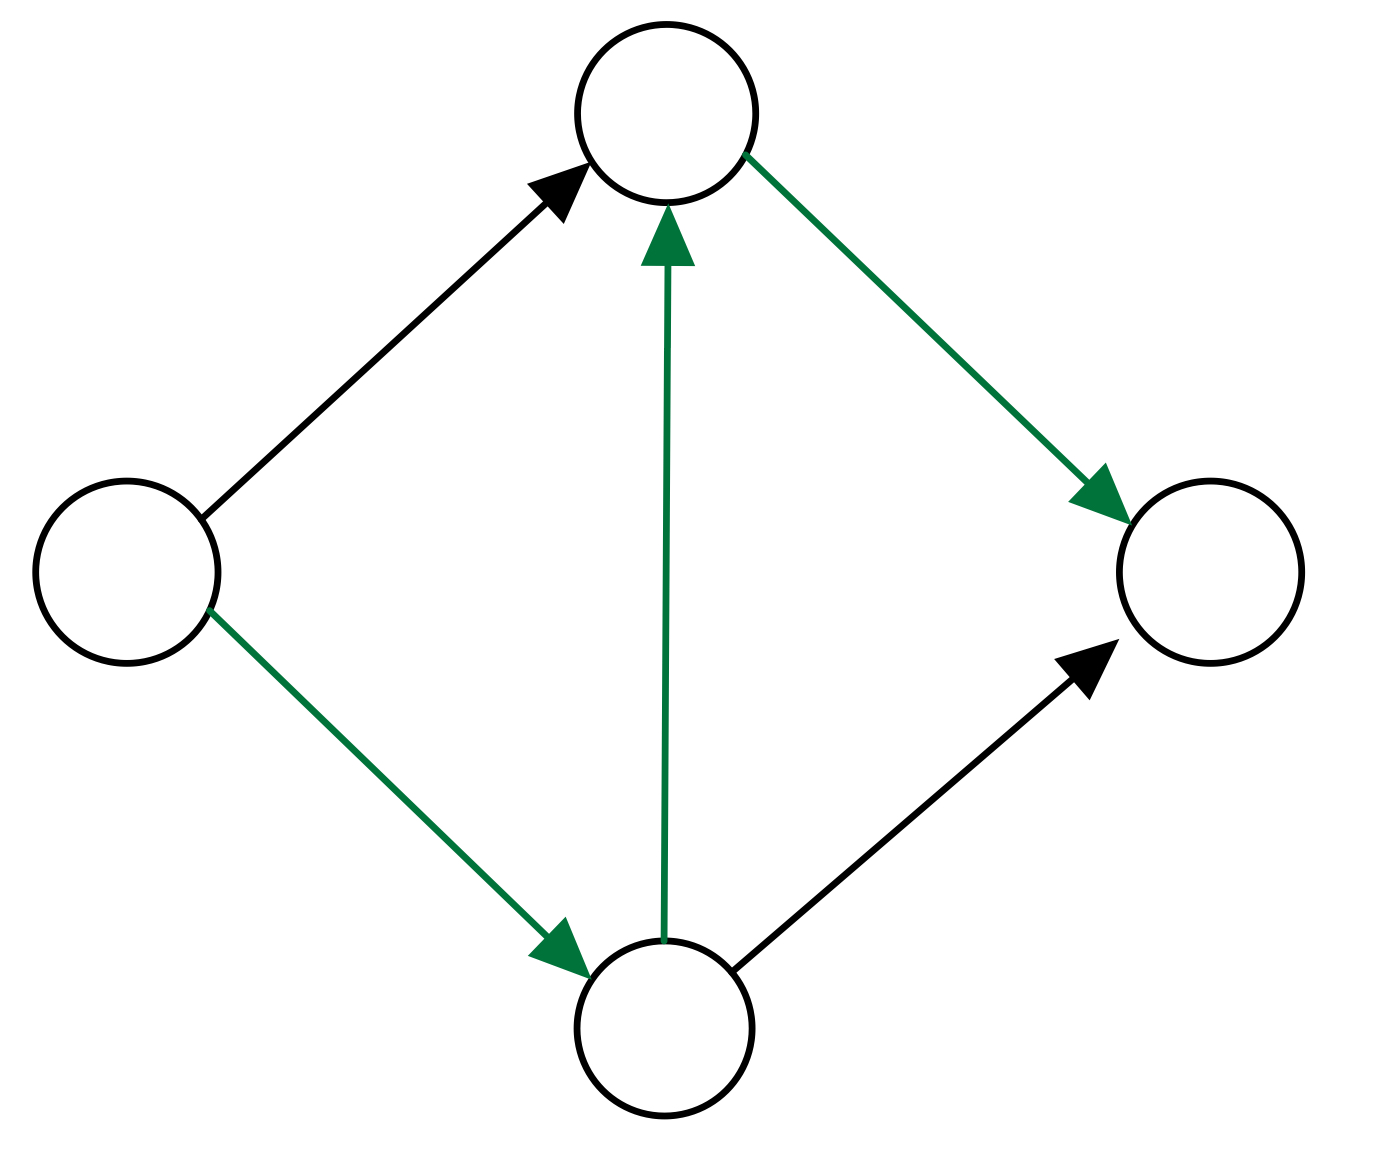
\includegraphics[scale = 0.15]{~/Study/3rdSem/Algorithms/Abstracts/images/lect03/blocking_flow.jpeg}
\end{example}

\begin{note}
	Блокирующий поток совершенно не обязательно наибольший.	
\end{note}

\subsection{Поиск блокирующего потока}

За $O(nm)$ \\

\textit{Забудем что у нас бывают обратные ребра.} \\
Идея проста, будем пускать поток пока получается, а для оптимизации учтем тот факт, что если мы уже однажды пытались пойти вдоль ребра, и узнали что после прохода по нему дойти до $t$ не получится, то нам не стоит идти по этому ребру снова. Это аналог метки used в DFS.

\newpage 

\begin{lstlisting}[language = C++]
	auto first_worthy_edge_num = vector<int>(); 
	/*first_worthy_edge[v] -- relative number of the first edge 
							  which is worth considiring from v. */

	long long dfs(int v, long long flow){
	//If we've followed the path and we can push the flow, we do it.

		if (v == t) return flow;

	//While there is at least one worthy edge.
		while (first_worthy_edge_num[v] < outbound[v].size()){
			auto cur_e = g[v][first_worthy_edge_num[v]];
		
		/*If there is some additional flow we can push and the edge is 
						 presented in initial network (is not reverse). */

		//We will code edge presence checker in Dinic's algorithm.
		if (edges[e].capacity > edges[e].flow && e is not reverse edge){
				auto next_flow = dfs(edges[e].to, 
				                     min(flow, edges[e].cap - edges[e].flow));


				if (next_flow > 0){
					edges[e].flow	 += next_flow;
					edges[e ^ 1].flow -= next_flow;

					return next_flow;
				}
			}
		
			++first_worthy_edge_num[v];
		}

		return 0;
	}
\end{lstlisting}

Тогда сам поиск блокирующего потока будет иметь вид
\begin{lstlisting}[language = C++]
	while ((auto x = dfs(s, inf)) != 0){
		blocking_flow += x;
	}
\end{lstlisting}

Алгоритм работает за $O(nm)$, ведь если главный вызов dfs (из main) суммарно сдвинул все номера интересных вершин на $k$, то dfs работал  $n + k$, так как каждое ребро либо нас устроило, и мы просто увеличили номер, либо оно нас устроило, и мы пошли в новую вершину, а сдвигать указатели долго мы не сможем, суммарно сдвигов будет не больше чем  $m$, а значит время работы $ =  n * $ кол-во запусков $+ m$, а каждый запуск насыщает хоть 1 ребро, при этом из-за отсутствия обратного ребра, ребра не рассыщаются. Значит имеем асимптотику  $O(nm)$

\subsection{Алгоритм Диница для поиска наибольшего потока }

За $O(n^2 m)$ \\

Пусть $G$ -- сеть. \\
$dist(s, v)$ -- кратчайшее расстояние между вершинами. \\

Определим слоистую сеть: \\
Вершина s. \\
Вершины с $dist$ 1 от s. \\
	... \\
Вершины на расстоянии k от s. \\

При этом оставим только ребра, идущие из меньшего уровня в следующий по порядку, то есть кратчайшие пути.

\textbf{Алгоритм} \\
\textit{Вспомним что у нас бывают обратные ребра.}\\
Пока не найден наибольший поток:
\begin{enumerate}
	\item Построим слоистую сеть.
	\item Пустим в ней произвольный блокирующий поток.
\end{enumerate}

\begin{prop}
	Алгоритм Диница находит наибольший поток.	
\end{prop}

\begin{proof} \ \\
	Теорема Форда-Фалкерсона учит нас что поток максимален $\iff$ в остаточной сети нет увеличивающего пути. Если наш алгоритм завершился, то есть не сумел пустить блокирующий поток в слоистой сети, значит в слоистой сети нет пути из $s$ в  $t$, а по построению слоистой сети, это значит что и в исходной сети пути из $s$ в  $t$.
\end{proof}

\begin{prop}
	Алгоритм Диница делает не более $n$	итераций.
\end{prop}

\begin{proof} \ \\
	Покажем что после каждой итерации $dist'(s, t) > dist(s, t)$. \\
	На каждом пути из $s$ в  $t$ есть хоть одно насыщенное ребро, ведь мы пустили блокирующий поток. (По определению блокирующего потока) \\
	После того как мы пустили блокирующий поток, у в слоистой сети исчезли некоторые ребра слева направо, а обратные ребра справа налево наоборот появились, значит расстояние в слоистой сети увеличилось, а значит увеличилось и расстояние в исходной сети.
\end{proof}


\subsection{Теоремы Карзанова.}%
\label{sub:Теоремы Карзанова.}

Зачастую асимптотика алгоритма Диница завышена, так как сеть в задаче имеет специфичный вид. Теоремы Карзанова помогают точнее оценить число итераций.

\begin{Def}
	\textbf{$C_{out}(v)$} $= \sum\limits_{u \in V} cap(v, u)$
	\textbf{$C_{in}(v)$} $= \sum\limits_{u \in V} cap(u, v)$
\end{Def}

\begin{note}
	Понятно что тогда через любую вершину течет не более чем $min(C_{in}(v), C_{out}(v))$
\end{note}

\begin{Def}
	\textbf{Общий потенциал сети $P$} $= \sum\limits_{v \in V, v \neq s, t} min(C_{out}(v), C_{in}(v))$
\end{Def}

\begin{lemma}
	В сети $G$ $l = dist(s, t) \leq \frac{P}{F} + 1$, где $F$ -- максимальный поток, $P$ -- общий потенциал. 
\end{lemma}
\begin{proof} \ \\
	Пусть $V_i = \{v: dist(s, v) = i\}$ \\
	Получилась слоистая сеть, в которой ребра есть только из  $V_i$ в  $V_{i + 1}$ \\
	Таким образом, если разрез и пересекает какое-либо ребро, то оно идет между слоями \\
	A cумма capacity ребер между слоями не меньше чем максимальный поток. \\ 
	$cap(\cup_0^i V_k, \cup_{i + 1}^l V_k) = \sum\limits_{x \in V_i, y \in V_{i + 1}} cap(x, y) \geq F$ \\
	Просуммируем это неравенство по всем $i$: \\
	$\sum\limits_{i = 0}^{l - 1} \sum\limits_{x \in V_i, y \in V_{i + 1}} cap(x, y) \geq (l - 1)F$ \\
	А сверху эту сумму можно оценить общим потенциалом сети, ведь сумма capacity ребер между слоями не может превышать сумму capacity ребер в одном слое, которая, в свою очередь, не превышает сумму потенциалов вершин в $V_i$. \\
	$P \geq (l - 1)F$
\end{proof}

\begin{lemma}
	После проталкивания потока $f$	в сети $G$, общий потенциал остаточной сети  $G_f$ равен общему потенциалу исходной сети.
\end{lemma}
\begin{proof} \ \\
	Когда мы проталкиваем поток $f$ вдоль ребер $(u, v)$ и $(v, w)$ по обратным ребрам проходит $-f$. \\
	Таким образом уменьшение $C_{in}(v)$ за счет потока по $(u, v)$ будет скомпенсировано увеличением  $C_{in}(v)$ за счет увеличения потока по обратному ребру  $(w, v)$.
\end{proof}

\begin{theorem}
	Число итераций алгоритма Диница в сети $G$ с целочисленными capacity --  $O(\sqrt{P})$
\end{theorem}
\begin{proof} \ \\
	Сделаем ровно $\sqrt{P}$ итераций, тогда $l \geq \sqrt{P}$, ведь, как мы уже знаем, каждая итерация увеличивает расстояние между $s$ и $t$ хоть на 1. \\
	Запишем утверждение первой леммы для остаточно сети после $\sqrt P$ итераций: \\
	$l \leq  \frac{P}{F_{ост}} + 1$, а $F_{ост} = F - f$, где $f$ -- то сколько потока удалось протолкнуть за прошедшие итерации. \\
	При это $f \geq \sqrt P$, ведь все capacity целочисленные, и мы не могли проталкивать меньше 1 единицы потока за итерацию. \\
	Таким образом получаем $F \leq 2\sqrt{P}$ 
\end{proof}
